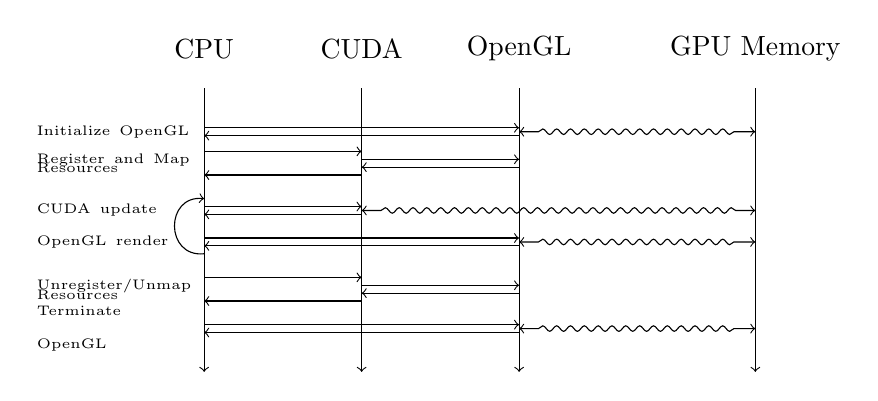
\begin{tikzpicture}[decoration = {snake,pre length=7pt,post length=7pt,amplitude=1pt,segment length=5pt}]
    % Arrows/timelines
    \draw[->] (0,0) -- (0,-3.6);
    \draw (0,0.5) node[anchor=center] {CPU};
    \draw[->] (2,0) -- (2,-3.6);
    \draw (2,0.5) node[anchor=center] {CUDA};
    \draw[->] (4,0) -- (4,-3.6);
    \draw (4,0.5) node[anchor=center] {OpenGL};
    \draw[->] (7,0) -- (7,-3.6);
    \draw (7,0.5) node[anchor=center] {GPU Memory};

    % Steps
    \draw[->] (0, -0.5) -- (4, -0.5);
    \draw[<->,decorate] (4, -0.55) -- (7, -0.55);
    \draw[<-] (0, -0.6) -- (4, -0.6);
    \draw (0, -0.55) node[anchor=east,text width=2cm] {{\tiny Initialize OpenGL}};

    \draw[->] (0, -0.8) -- (2, -0.8);
    \draw[->] (2, -0.9) -- (4, -0.9);
    \draw[<-] (2, -1.0) -- (4, -1.0);
    \draw[<-] (0, -1.1) -- (2, -1.1);
    \draw (0, -0.95) node[anchor=east,text width=2cm] {\shortstack[l]{\tiny Register and Map\\[-4pt]\tiny Resources}};

    \draw[->] (0, -1.5) -- (2, -1.5);
    \draw[<->,decorate] (2, -1.55) -- (7, -1.55);
    \draw[<-] (0, -1.6) -- (2, -1.6);
    \draw (0, -1.55) node[anchor=east,text width=2cm] {{\tiny CUDA update}};

    \draw[->] (0, -1.9) -- (4, -1.9);
    \draw[<->,decorate] (4, -1.95) -- (7, -1.95);
    \draw[<-] (0, -2.0) -- (4, -2.0);
    \draw (0, -1.95) node[anchor=east,text width=2cm] {{\tiny OpenGL render}};

    \draw[->] (0, -2.1) .. controls (-0.5,-2.15) and (-0.5,-1.35) .. (0, -1.4);

    \draw[->] (0, -2.4) -- (2, -2.4);
    \draw[->] (2, -2.5) -- (4, -2.5);
    \draw[<-] (2, -2.6) -- (4, -2.6);
    \draw[<-] (0, -2.7) -- (2, -2.7);
    \draw (0, -2.55) node[anchor=east,text width=2cm] {\shortstack[l]{\tiny Unregister/Unmap\\[-4pt]\tiny Resources}};

    \draw[->] (0, -3.0) -- (4, -3.0);
    \draw[<->,decorate] (4, -3.05) -- (7, -3.05);
    \draw[<-] (0, -3.1) -- (4, -3.1);
    \draw (0, -3.05) node[anchor=east,text width=2cm] {{\tiny Terminate OpenGL}};
\end{tikzpicture}